
\documentclass[]{spie}  %>>> use for US letter paper
%\documentclass[a4paper]{spie}  %>>> use this instead for A4 paper
%\documentclass[nocompress]{spie}  %>>> to avoid compression of citations

\renewcommand{\baselinestretch}{1.0} % Change to 1.65 for double spacing

\usepackage{amsmath,amsfonts,amssymb}
\usepackage{graphicx}
\usepackage[colorlinks=true, allcolors=blue]{hyperref}
% user added packages
\usepackage{xcolor}
\usepackage{adjustbox}
\usepackage{ulem}
%\usepackage{natbib}

% user added commands
\newcommand{\comr}[1]{\textcolor{red}{#1}}
\newcommand{\comb}[1]{\textcolor{blue}{#1}}
\newcommand{\como}[1]{\textcolor{orange}{#1}}
\newcommand{\dgr}{$^\circ$}

% journal abbreviations for bibtex
\def\aap{\it{A\&A}}
\def\apj{\it{ApJ}}                 % Astrophysical Journal
\def\apjl{\it{ApJ}}                % Astrophysical Journal, Letters
\def\apjs{\it{ApJS}}               % Astrophysical Journal, Supplement
\def\ao{\it{Appl.~Opt.}}           % Applied Optics


\title{Optical Design of PICO, a Concept for a Space Mission to Probe Inflation and Cosmic Origins}

\author[a\dag]{Karl Young}      %UMN
\author[b]{Marcelo Alvarez}  % University of California Berkeley, USA
\author[c]{Nicholas Battaglia}  %  Princeton
\author[d]{Jamie Bock}       % Caltech
\author[e]{Jullian Borrill}  % LBNL
\author[f]{David Chuss}  % Villanova  University, USA
\author[g]{Brendan Crill}    % JPL
\author[h]{Jacques Delabrouille}  % APC
\author[i]{Mark Devlin}  % U Penn
\author[j]{Laura Fissel}  % NRAO, USA
\author[k]{Raphael Flauger} % UC san diego 
\author[l]{Daniel Green}  % University of Toronto, Canada
\author[g]{Kris Gorksi}  % JPL
\author[a]{Shaul Hanany} % UMN
\author[m]{Richard Hills} % Cambridge
\author[n]{Johannes Hubmayr} % NIST, USA
\author[o]{Bradley Johnson}  % Columbia University, New York
\author[c]{Bill Jones}  %Princeton 
\author[p]{Lloyd Knox}  % UC Davis
\author[q]{Al Kogut}  %Goddard
\author[g]{Charles Lawrence}  % JPL
\author[r]{Tomotake Matsumura} % IPMU, Tokyo
\author[g]{Jim McGuire}  % JPL
\author[s]{Jeff McMahon}  % U of MI
\author[g]{Roger O'Brient} %JPL
\author[a]{Clem Pryke}  % UMN
\author[g]{Brian M. Sutin}  % JPL
\author[a]{Xin Zhi Tan}  % UMN
\author[g]{Amy Trangsrud}  % JPL
\author[a]{Qi Wen}  % UMN
\author[t]{Gianfranco de Zotti}  % padova, Osservatorio Astronomico di Padova, Italy


\affil[a]{University of Minnesota, USA}
\affil[b]{University of California Berkeley, USA}
\affil[c]{Princeton University, USA}
\affil[d]{California Institute of Technology, USA}
\affil[e]{Lawrence Berkeley National Laboratory, USA}
\affil[f]{Villanova  University, USA}
\affil[g]{Jet Propulsion Laboratory, California Institute of Technology, USA}
\affil[h]{Laboratoire AstroParticule et Cosmologie and CEA/DAP, France}
\affil[i]{University of Pennsylvania, USA}
\affil[j]{National Radio Astronomy Observatory, USA}
\affil[k]{University of California San Diego, USA}
\affil[l]{University of Toronto, Canada}
\affil[m]{Cavendish Laboratory, University of Cambridge, UK}
\affil[n]{National Institute of Standards and Technology, USA}
\affil[o]{Columbia University, USA}
\affil[p]{University of California Davis, USA}
\affil[q]{Goddard Space Flight Center, USA}
\affil[r]{Kalvi IPMU, University of Tokyo, Japan}
\affil[s]{University of Michigan, USA}
\affil[t]{Osservatorio Astronomico di Padova, Italy}

\authorinfo{$^\dag$E-mail: kyoung@astro.umn.edu, Telephone: 1 612 626 9149}

% Option to view page numbers
\pagestyle{empty} % change to \pagestyle{plain} for page numbers   
\setcounter{page}{1} % Set start page numbering at e.g. 301
 
\begin{document} 
\maketitle

\begin{abstract}

The Probe of Inflation and Cosmic Origins (PICO) is a probe-class mission concept currently under study by NASA.  
PICO will probe the physics of the Big Bang and the energy scale of inflation, constrain the sum of neutrino masses, 
measure the growth of structure in the universe, and constrain its reionization history by making full sky maps of the 
cosmic microwave background with sensitivity 70 times higher than the Planck space mission. With bands at 
21-799~GHz and arcmin resolution at the highest frequencies, PICO will make polarization maps of galactic synchrotron 
and dust emission to observe the role of Galactic magnetic fields in galactic evolution and star formation. 
We describe the current state of the PICO instrument design.  We discuss the choice of optical system, which is based on 
an open-Dragone telescope that, to our knowledge, has not been used for mm-wave astrophysical observations. 
We also present the focal plane design, a white noise model of the instrument, and the expected noise level. 

\comr{did you review the abstract? does it accurately represent the contents of the paper? Is it highlighting the unique and new 
things you are reporting? Is it quantitative? } \como{In order; yes, yes, I think so, and somewhat.}

\end{abstract}

% Include a list of keywords after the abstract 
\keywords{Cosmic microwave background, cosmology, mm-wave optics, polarimetry, instrument design, satellite, mission concept}


\section{INTRODUCTION}
\label{sec:intro}  


Over the last decade NASA's astrophysics division has funded design and construction of space missions that are either Explorer-class, 
with cost cap of $\leq \$250$M or Flagship-class that cost above \$1B. 
To study the science opportunities available at intermediate costs, NASA initiated studies of Probe-class missions with cost window 
between \$400M and \$1B.  We are conducting one these studies for a mission called the Probe of Inflation and Cosmic Origins (PICO). 
A paper by Sutin et al.\cite{brian_spie}\ in these proceedings gives an overall review of PICO and the scientific motivation.  
This paper describes the design of the telescope and focal plane and gives 
our current best estimates for the sensitivity of the instrument. The mission study is not complete; the final report 
is due in December 2018. Therefore, the quantitative assessments we provide are temporary in nature and subject to revision. 
Even so, the design is fairly mature and we do not expect significant changes. 
Values in this paper, such as component temperatures and detector noise levels,  
are current best estimates. They are not finalized mission requirements. 

% \sout{Astrophysical observations in the  millimeter and sub-millimeter region of the electromagnetic spectrum contain a wealth of 
% information about the formation, evolution, and structure of the Universe.  
% The polarization and temperature anisotropies of the cosmic microwave 
% background (CMB) encode fundamental physics information relating to the epoch of inflation, the mass of neutrinos,  
% and the number of relic light particles in the early Universe. They also contain information about the formation of 
% the first stars, galaxies, and clusters, as well as information on emission from the innermost regions of radio source jets.
% Information about the role of magnetic fields in star formation and galactic evolution is obtainable 
% by observing the polarized emission of Galactic dust, which 
% traces magnetic fields, at high resolution. Targeting both of these regimes, PICO will survey the entire sky with 
% unprecedented polarization sensitivity 
% in 21 bands centered at 21--799~GHz.  Details of these science targets and expected constraints from PICO 
% are in a companion paper, Sutin~et~al.\cite{brian_spie} 
% In this paper we discuss the mission's optical system, focal plane, and sensitivity.}

\section{MISSION AND SPACECRAFT}
\label{sec:spacecraft}

PICO will conduct scientific observations for five years from an orbit around the Earth-Sun L2 Lagrange point. The design had
21 bands centered at 21--799~GHz.  The spacecraft design impacted 
the optical design and sensitivity in two primary ways; volume constraints limited the physical size of the telescope and optical component 
temperatures impacted noise levels.  

The maximum diameter of the spacecraft was limited by the SpaceX's Falcon 9 launch vehicle, which carried payloads up to 4.6~m in diameter. 
This diameter limited the V-groove shields' size, which, along with the scan strategy, defined the `shadow cone' in Figure~\ref{fig:cad}.  
The shadow cone was the volume protected from solar illumination, and all optical components were contained within it. The shadow cone and 
inner V-grooves defined an available volume for the telescope.  We opted not to use deployable shields as they presented added cost 
and risk which outweighed the benefits. The thermal model indicated the temperatures of the optical elements as given in Figure~\ref{fig:cad}. 
The primary reflector was passively cooled, while the optics box, secondary reflector, and focal plane were actively cooled; Sutin~et~al.\cite{brian_spie}
gives more details of the thermal system. 

\begin{figure} [ht]
\begin{center}
%\begin{tabular}{c} %% tabular useful for creating an array of images 
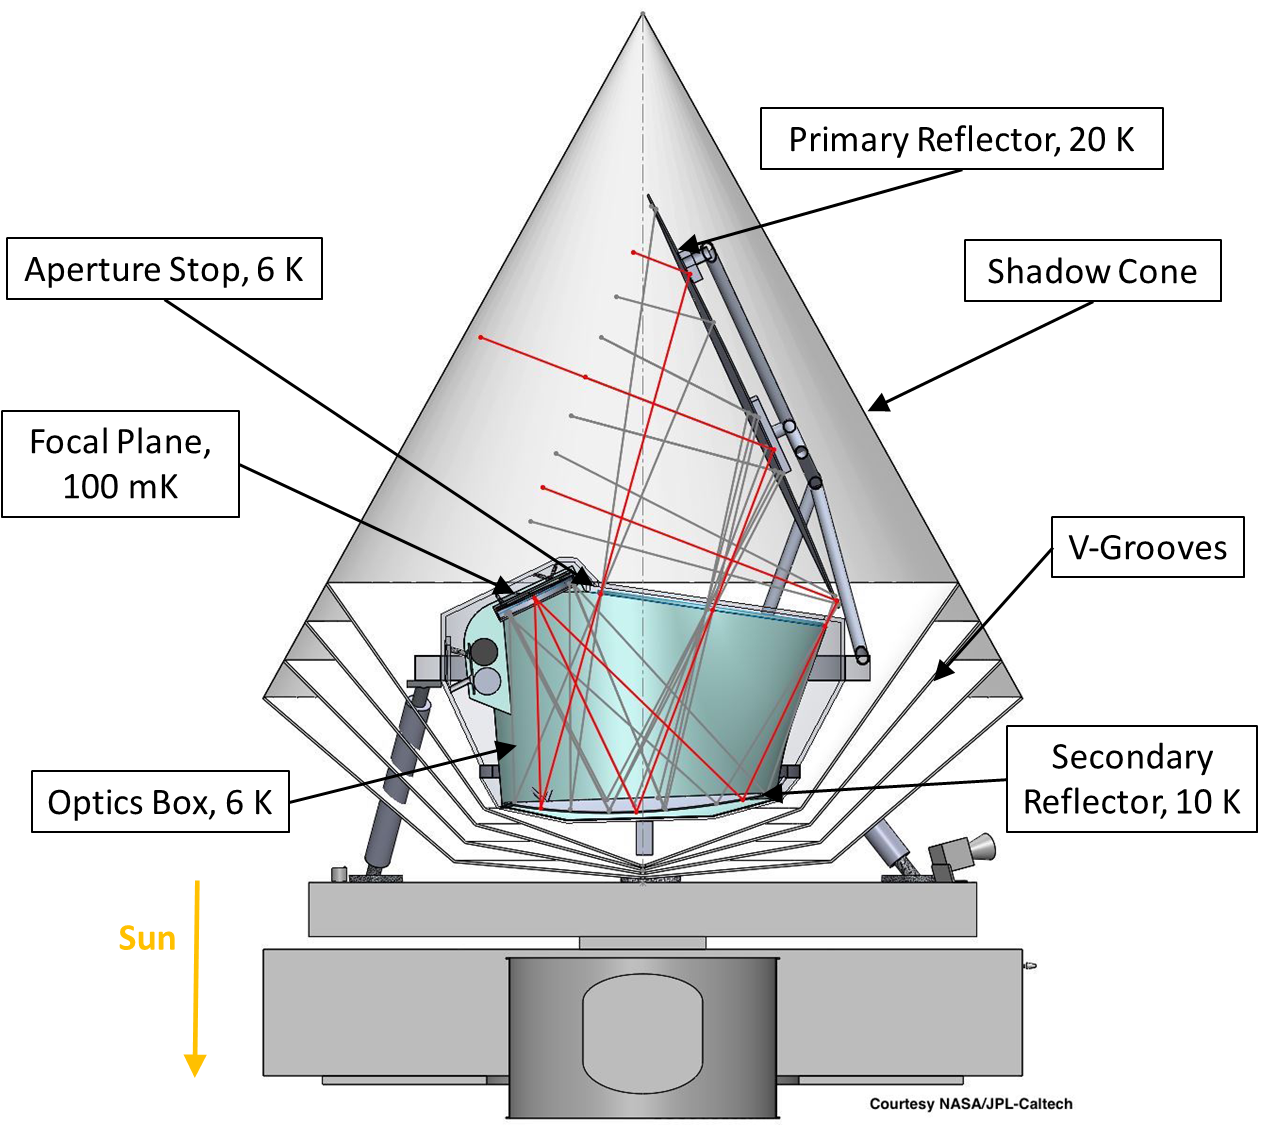
\includegraphics[height=9cm]{PICO_CAD_annotated.png}
%\end{tabular}
\end{center}
\caption { \label{fig:cad} 
\sout{Mechanical design of the PICO satellite. Components relevant to this paper are labeled, for other details see Sutin~et~al.\cite{brian_spie}}
The symmetry axis of the satellite precesses around the satellite-sun axis (orange arrow) with an angle of 26 deg \comr{figure is confusing; show the spin 
axis; show the sun along the shadow cone; show the boresight explicitly; show the 26 and 69 degrees}. This precession defines the 
shadow cone which is shown in light gray.
}
\end{figure} 

% \begin{itemize}
% \item Sketch out satellite systems. Include CAD model figure and table of system parameters
% \subitem thermal systems and surface temperatures (NOTE! a bunch of these in Brian's paper don't match what we have used.  filters 1 K, stop 4.5-6 K, secondary 10 K, Primary 20 K, maybe others. Unclear how much of this will be in final version.
% \subitem sunshields and scan strategy
% \subitem observing frequency ranges 
% \item Summarize mission 
% \subitem L2 orbit, for earth-moon viewing angles
% \subitem 5 yrs active time frame
% \subitem launch vehicle is Falcon 9 
% \end{itemize}


\section{OPTICAL SYSTEM}
\label{sec:optics}

The choice of telescope design was driven by a combination of science
requirements and the physical limits discussed in Section~\ref{sec:spacecraft}.  The science requirements were: a large diffraction 
limited field of view (DLFOV)\footnote{ We consider an area in the FOV diffraction limited when the Strehl ratio is 
larger than 0.8.} sufficient to support $\mathcal{O}(10^4)$ detectors, arcminute resolution at 800~GHz, low 
instrumental polarization, and low sidelobe response. Additionally, 
the transition edge sensor bolometers baselined for PICO require a telecentric focal plane which is sufficiently flat that it 
can be tiled by 10~cm detector wafers without reduction in optical quality. 

To increase aperture efficiency and reduce sidelobes we concentrated on off-axis optical designs.
More than 30 years ago Dragone analyzed the 
performance of several off-axis systems and found solutions with low cross-polarization at the center of the field 
of view and with astigmatism, or astigmatism and coma, canceled to first order.\cite{dragone,dragone_coma,dragone1983} These
systems also had no cross-polarization at the center of the field of view. 
A number of recent CMB instruments used off-axis systems, and several 
began the design optimization with systems based on designs by
Dragone\cite{planck2000_optics,ACT2011_optics,SPT2008_optics,core2018_inst,LB2016_optics,parshley_ccat_spie}. 
For PICO we began 
the optimization with a two-reflector Dragone system that, to our knowledge, has not been implemented in CMB instruments before. 
We call it an `open-Dragone' because of its overall geometry and in contrast to the widely used `cross-Dragone', see Figure~\ref{fig:ray}. 
We used a 1.4~m entrance aperture as this aperture diameter satisfied the science requirements.

We considered two additional Dragone systems, a Gregorian Dragone and a cross-Dragone, and compared the 
relative performance of all three systems in terms of DLFOV, compactness, and rejection of sidelobes.  
Compared to the open-Dragone, the Gregorian had half the DLFOV for the same $F$-number and could not  
support $\mathcal{O}(10^4)$ detectors. It was therefore rejected.  
The cross-Dragone had roughly $4\times$ the DLFOV of the open-Dragone, 
but was more difficult to pack inside the spacecraft volume while avoiding the known sidelobes shown in Figure~\ref{fig:sidelobes}.
We found that the largest cross-Dragone which meets the PICO volume constraints had 
a 1.2~m aperture and an $F$-number of 2.5, while the largest open-Dragone aperture was 1.4~m with an $F$-number of 1.42. The larger 
$F$-number of the cross-Dragone system implied a larger physical focal plane, and therefore higher mass and cost, 
for the same number of pixels. 
For the PICO case, we concluded that the advantages of a low $F$-number and easily baffled sidelobes made the open-Dragone a good starting  
point for further optimization. 

%A cross-Dragone will always have a larger $F$-number 
%than an open-Dragone of the same aperture size, because the cross-Dragone focal length must be long enough that the focal plane 
%does not block the primary mirror. } 
% \comr{Can you really make such a general claim? }
%\comr{why does it 'always' have larger F? Can make a smaller F, no?}. \como{The smallest $F$-number of a crossed system is about 2. The focal length has to be long so the focal plane doesn't block the primary. You could make an open with F > 2, but you can't make a crossed system with F < 2.}

\begin{figure} [ht]
\begin{center}
%\begin{tabular}{c} %% tabular useful for creating an array of images 
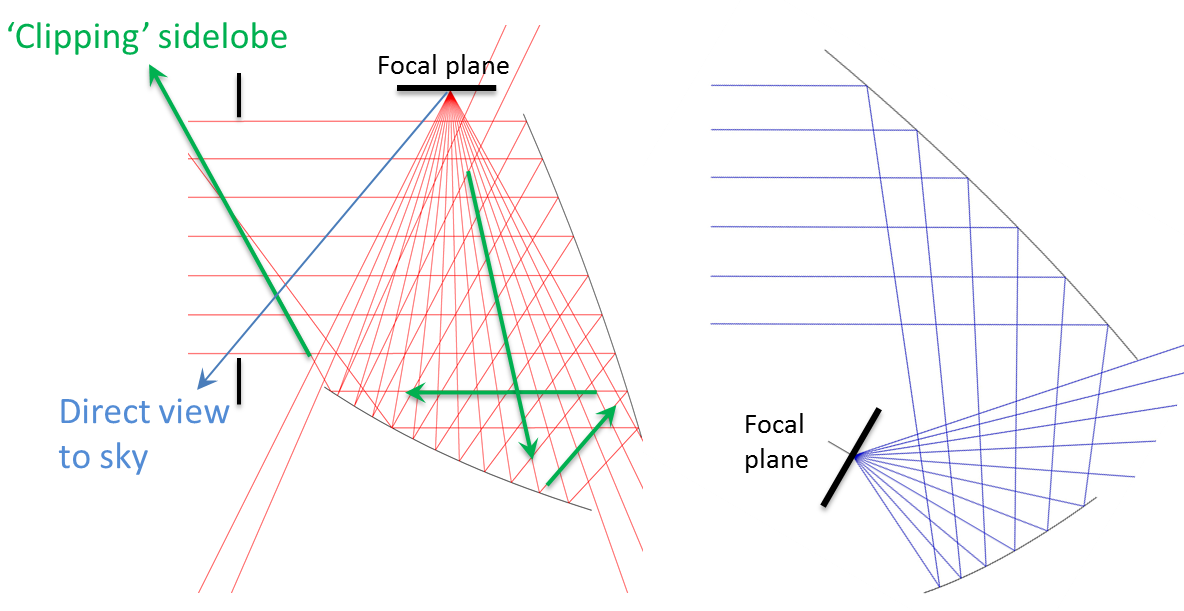
\includegraphics[height=6.5cm]{sidelobes.png}
%\end{tabular}
\end{center}
\caption { \label{fig:sidelobes} 
Comparison of sidelobes for a cross-Dragone (left) and an open-Dragone (right) \comr{please add labels to Figure as well}.  
Rays are traced from the center of the focal plane toward the sky \comr{same angular opening of rays?}.
For both systems spillover around the secondary is straightforward to mitigate with absorptive baffles \comr{show sketch of such baffles?}.  
However, the rays labeled `sidelobe' and `direct view to 
sky' in the cross-Dragone system present added challenges. The challenges can be mitigated---with a long forebaffle or larger $F$-number (see
for example Matsumrua et al.\cite{LB2016_optics}---but
doing so increases the overall physical size of the system, which is problematic in the PICO case.}
\end{figure} 

We designed the initial open Dragone following Granet's method\cite{granet2001}. 
We began with a solution with $F=1.42$, a 1.4~m aperture (that was verified to satisfy the volume constraints), and a large 
DLFOV.  We forced a circular aperture stop 
between the primary and secondary reflectors and numerically optimized its angle and position to obtain the 
the largest DLFOV.  The stop diameter was chosen such that, for the center feed, it projected a 
1.4~m effective aperture onto the primary. 
Adding a stop in this way increased the size of the primary reflector, because 
different field angles illuminated different areas on the reflector.
Actively cooling the aperture stop, however, reduced detector noise, and the stop shielded the 
focal plane from stray radiation. At this stage the system still met 
the Dragone condition and is defined by the `Initial Open-Dragone' parameters in Table~\ref{tab:optics}.

In his publications Dragone provides a prescription to eliminate coma
in addition to the cancellation of astigmatism provided by the baseline designs.\cite{dragone_coma} The corrections 
involve adding distortions to the primary and secondary reflectors 
which are proportional to $r^4$ where $r=0$ is at the chief ray impact point on each reflector. 
We thus attempted to increase the DLFOV using two methods. 

In `Method1', one of the coauthors (RH) used Zemax to add Zernike 
polynomials to the base conics which described the reflectors. These Zernike polynomials were offset from the symmetry axis of the conic 
by $624.2$~cm for the primary and $76.1$~cm for the secondary.  
This placed the origin of polynomials at the chief ray impact point for each reflector. 
Inspired by the Dragone corrections, all Zernike terms up to fourth order and the first fifth order term were allowed to vary. 
The optimization metric was minimization of the rms spot diameter at 
the following locations: the center of the FOV, $\pm2$~deg in Y, and $\pm4$~deg in X. The center of the FOV was given a weight of 100
while each outer point was given a weight of 1. To constrain the optimization, the X and Y 
effective focal lengths were held fixed as was the impact point of the chief ray on the focal plane. 
This optimization step increased the DLFOV
by factors of 1.15, 2.4 and 10.5 at 21, 155 and 799~GHz, respectively. 
We further increased the DLFOV by approximately 50\% at all frequencies by including a curved focal surface and rerunning the optimization.
A small ($\sim$4\%) additional gain in DLFOV was achieved by adding Zernike terms 
up to sixth order, allowing the secondary to focal surface distance to vary, adding a weighted constraint on the effective focal length, 
and adding fields with weight of 0.01 to the rms spot diameter metric at $\pm7.5$~deg in Y and $+15$~deg in X. 
These additional fields were necessary to constrain the corrections at the reflector edges.

% \comr{The other method by Richard has the first step of converting the conics into an on axis XY polynomial representation. Then a similar procedure is followed.  It is less well behaved during optimization.  This second Richard method is what I replicated in CodeV.}
% \comb{is this 'other method' = method2? or is it 1b? \como{KY: My method is 1b and not discussed here.}}


\begin{figure} [ht]
\begin{center}
%\begin{tabular}{c} %% tabular useful for creating an array of images 
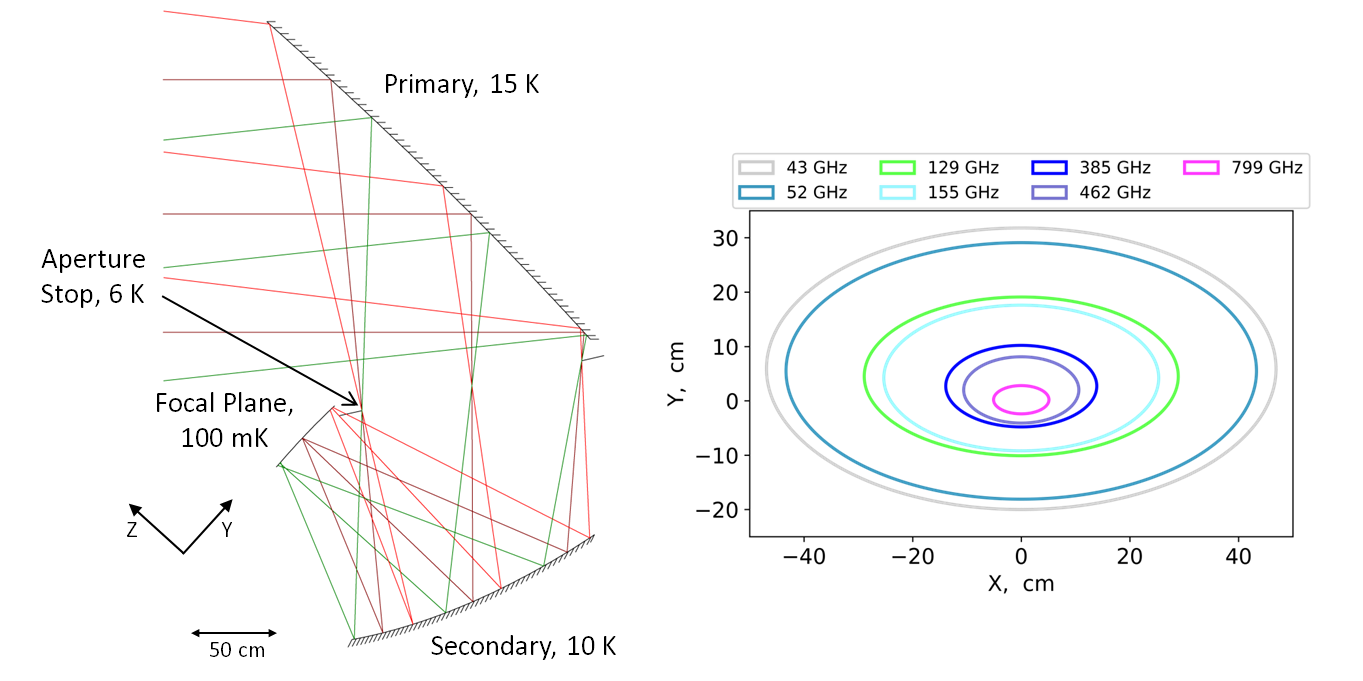
\includegraphics[height=7.5cm]{jpl_ray_strehl.png}
%\end{tabular}
\end{center}
\caption { \label{fig:ray} \label{fig:strehl} 
Raytrace (left) and Strehl~$=0.8$ contours (right) for the PICO optical design.
}
\end{figure} 

\begin{table}[ht]
\centering
\caption{Telescope geometric parameters  \comr{ADD F\# to Table} \label{tab:optics}}

\begin{adjustbox}{width=1.05\textwidth}
\hspace{-1cm}
\begin{tabular}{|l|llll||ll|}
\hline
\multicolumn{5}{|c||}{PICO optical system}                                    & \multicolumn{2}{c|}{Initial Open-Dragone$^b$}     \\ \hline
                          & Primary           & Secondary    & \multicolumn{2}{c||}{Telescope parameters$^b$} & \multicolumn{2}{c|}{Fundamental design parameters}  \\
Reflector size$^a$ (cm)      & $270 \times 205$ & $160 \times 158$ & Aperture (cm)           & 140      & Aperture (cm)                  & 140   \\
Radius of curvature (cm)  & $\infty$         & 136.6             & $F$-number             & 1.42     & $\theta_0$ (deg)           & 90    \\
Conic constant, $k$       & 0                 & -0.926            & h (cm)                    & 624.2    & $\theta_e$ (deg)           & 20    \\
Normalization radius (cm) & 524.8             & 194.1             & $\alpha$ (deg)            & 74.2     & $\theta_p$ (deg)           & 140   \\
4th Zernike Coefficient (cm)  & 2018.4            & -61.1             & $\beta$  (deg)            &  62.3    & L$_m$ (cm)                     & 240   \\
9th Zernike Coefficient (cm)  & -37.0             & 16.7              & L$_m$ (cm)                &   229.3  &                                &         \\
10th Zernike Coefficient (cm) & -2919.8           & -15.1             & L$_s$ (cm)                &   140.5  & \multicolumn{2}{c|}{Derived parameters} \\ 
11th Zernike Coefficient (cm) & -1292.7           & 22.3              &                           &          & $F$-number                     & 1.42  \\   
12th Zernike Coefficient (cm) & 120.6             & -3.8             &   \multicolumn{2}{c||}{Focal Surface}  & h (cm)                         & 624.2 \\   
13th Zernike Coefficient (cm) & -74.5             & 4.9               & Ellipse major axes (cm)   & 69 x 45  & $\alpha$ (deg)                 & 38.6  \\   
19th Zernike Coefficient (cm) & -75.8             & 3.4               & Ellipse major axes (deg)  & 19 x 13  & $\beta$  (deg)                 & 101.4 \\   
20th Zernike Coefficient (cm) & -398.9            & 6.3               & Radius of curvature (cm)  & 455      & L$_s$ (cm)                     & 122.2 \\   
21st Zernike Coefficient (cm) & -319.5            & 23.3              &                           &          & Primary, $f$ (cm)              & 312.1 \\   
22nd Zernike Coefficient (cm) & -276.6            & -8.5              &                           &          & Secondary, $a$ (cm)            & 131   \\   
23rd Zernike Coefficient (cm) & -201.6            & -3.2              &                           &          & Secondary, $e$                 &  1.802  \\
24th Zernike Coefficient (cm) & -127.4            & -1.9              &                           &          &                                &       \\
25th Zernike Coefficient (cm) & -55.0             & 0.1               &                           &          &                                &       \\\hline
\multicolumn{7}{l}{\footnotesize  $^a$ The maximum physical size of the reflectors.}\\
\multicolumn{7}{l}{\footnotesize  $^b$ Telescope parameters follow the definitions in Granet 2001.\cite{granet2001}} \\
\end{tabular}
\end{adjustbox}
\end{table}


%To increase the optical performance we use CodeV to numerically optimize the system.  
In `Method2' another coauthor (JM) used 
%\comr{why is JM doing stuff in the present, while RH had done stuff in the past? please do all in the past} 
CodeV and allowed additional geometric parameters of the system to vary.  To adjust the 
reflector shapes, we added Zernike polynomial corrections to the conic surfaces which defined the two reflectors.
The Zernike polynomials were defined in the same coordinate systems as the base conics.  
We varied the 4th and 9th-13th Zernike coefficients. We allowed the focal surface curvature 
and focal surface to secondary distance L$_s$ to vary.  The primary-secondary distance L$_m$, primary offset $h$, 
and the primary and secondary rotation angles, $\alpha$ and $\beta$, were varied as well.  The optimization 
metric was the rms spot diameter across the field of view, with weighted constraints requiring telecentricity and 
maintaining the X- and Y-focal lengths.  We added Lagrange constraints 
to enforce beam clearances and place an upper limit on overall system size.  Once the optimization converged to 
an acceptable optical system, we added higher order Zernike terms, 19th-25th, and refined 
the reflector shapes using the same metric and constraints. 
The current PICO optical design is from the Method2 optimization procedure.  % Tense of this sentence is odd. "The design is" makes sense in terms of the paper structure, just as I would say 'Figure 1 shows'.  However in 5 yrs "The design is" will certainly be an incorrect statement.  Including 'current' avoids this somewhat by qualifying the status of the design.

Figure~\ref{fig:compare} shows that Method2 greatly increased the DLFOV relative to the initial open-Dragone design.  
The DLFOV increased by factors of 1.9, 3.8, 4.3, and 4.6 at 21, 129, 155, and 799~GHz, respectively.  
%\comr{what is the improvement relative to the RH approach?}
The most important gain was at frequencies of 129 and 155~GHz. We used this extra area to add 
more C and D pixels, see Figure~\ref{fig:bands} and Section~\ref{sec:focalplane}. The C and D pixels contained the bands 
most sensitive to the CMB, and adding hundreds of these pixels into the focal plane  
gave PICO unprecedented levels of CMB sensitivity. 
Method2 gave somewhat better performance at lower 
frequencies with a DLFOV 1.11 and 1.15 times larger than Method1 at 21 and 155~GHz, respectively.
At 799~GHz Method2 gave DLFOV only 0.3 times that of Method1's area, but the DLFOV still satisfied our science 
requirements. 
Figure~\ref{fig:compare} also shows that Method2 reduced the overall telescope volume and gave more 
physical margin relative to the shadow cone.

The geometric parameters of the PICO optical system are given in Table~\ref{tab:optics}. The 
system was diffraction limited for 799~GHz at the center of the field of view. At 155~GHz the 
DLFOV was 82.4~deg$^2$ and the total throughput at 20~GHz was 910 cm$^2$sr. 
Figure~\ref{fig:strehl} shows Strehl of 0.8 contours for all pixel types.
The slightly concave focal surface, which had a radius of curvature of 4.55~m, was telecentric to 
within 0.12~deg across the entire FOV.

\begin{figure} [ht]
\begin{center}
%\begin{tabular}{c} %% tabular useful for creating an array of images 
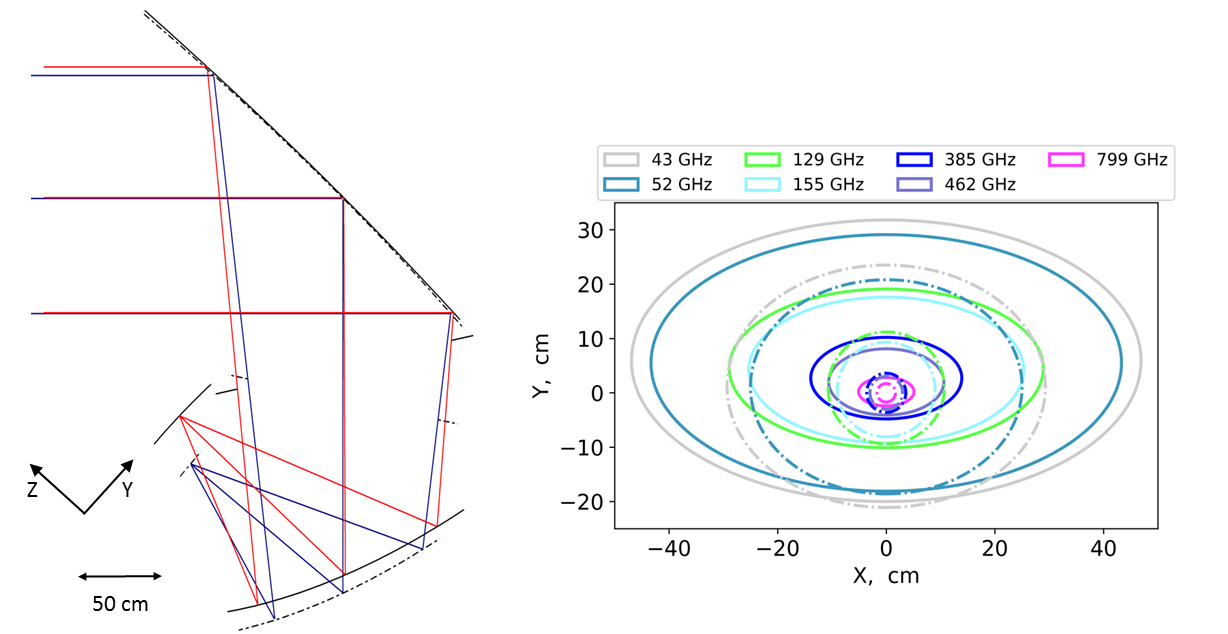
\includegraphics[height=7cm]{jpl_vs_V3D.png}
%\end{tabular}
\end{center}
\caption { \label{fig:compare} 
Comparison between the open-Dragone optimized using method two and the initial open-Dragone.  
The ray traces (left) are aligned at the chief ray impact point on the primary. 
The \comb{final optical system, optimized with Method2 (red rays, solid reflectors),} is smaller in the vertical direction 
than the unoptimized version \comr{original dragone or Method1?} (blue rays, dash-dot reflectors). The overlaid Strehl~$=0.8$ contours 
(right) show the improvement at all frequencies in the optimized (solid lines) system over the unoptimized (dash-dot lines) system. 
\comr{same question? Perhaps show all three options?}
}
\end{figure} 

An additional benefit of the optimization was the concave focal surface. The open-Dragone's focal surface is naturally curved.  Matching this 
curvature reduced defocus, increased the DLFOV, and increased telecentricity.  The unoptimized system was telecentric to within 
2.5~deg while the optimized version was telecentric to within 0.12~deg. If the focal surface was too strongly curved tiling it with flat detector 
wafers would result in large defocus at the edges of these wafers.  This was not the case for PICO. The focal surface radius of curvature, 4.55~m, 
resulted in a defocus of 0.1~mm at the edge of a 10~cm wafer. 



\section{FOCAL PLANE}
\label{sec:focalplane}

Modern mm/sub-mm bolometers are photon noise limited. An 
effective way to increase sensitivity is to increase the number of detectors in the focal surface. %% facts are always in present tense.
The PICO focal surface had 12,996 detectors, 175 times the number flown on \textit{Planck}. PICO achieved this by 
having a large DLFOV and using multichroic pixels (MCPs)\cite{Suzuki2014_samps,datta2014_mcp}. 
The MCP architecture assumed for PICO had three bands per pixel with two single polarization transition 
edge sensor (TES) bolometers per band and therefore six bolometers per pixel. 
We assumed the MCPs were coupled to free space using lenslets and sinuous antennae \cite{Suzuki2014_samps}, 
but the pixel sizes, numbers, and spacing will not change significantly 
if horn or phased array coupling is used instead.

PICO had 21 overlapping bands with centers spanning the range 21--799~GHz. The bands were divided amongst 
nine pixel types labeled A to I; see Figure~\ref{fig:bands}. 
%These bands provide the broad fequency coverage needed to seperate the CMB, Galactic dust, and various foregrounds using their differing spectra.  \comr{no. it is needed to achieve all of our science goals. separating foreground is only one of the goals of the broad frequency coverage.}
The 25\% fractional bandwidth was broader than the interband spacing causing neighboring bands to 
overlap and requiring them to be in separate pixels. 
%For example, bands 1, 3, and 5 are in pixel A while bands 2, 4, and 6 are in pixel B.  This 
%complicates the pixel design and focal plane layout, but allows broader bands which increases total sensitivity.  
%\comb{Be more succinct. A paper is not a tutorial. I don't agree that it leads to more complications}
The exceptions to the MCP architecture were the highest three bands, because they were above the superconducting 
band gap of the niobium used for transmission lines, antennae, and filters in MCPs.  
For bands G, H, and I, we assumed feedhorn-coupled polarization sensitive bolometers. The technology has high TRL 
as it has been used successfully with 
\textit{Planck}\cite{planck2010_hfi} and Herschel SPIRE\cite{spire2010}.

\begin{figure} [ht]
\begin{center}
%\begin{tabular}{c} %% tabular useful for creating an array of images 
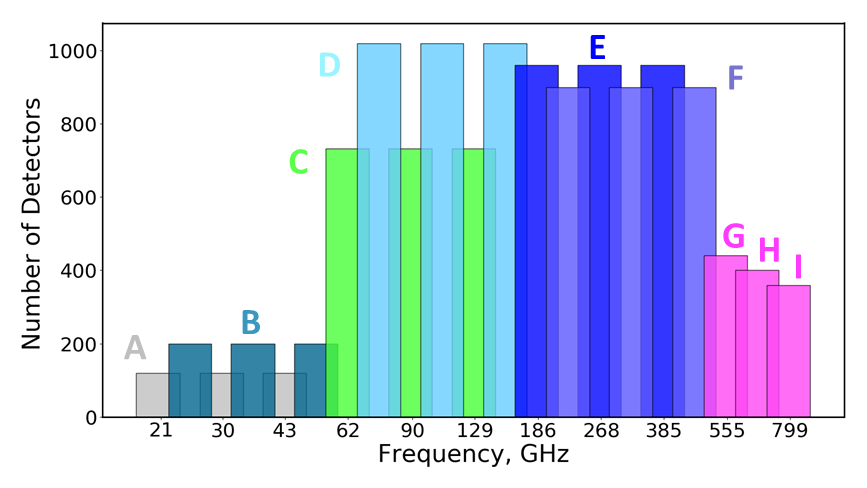
\includegraphics[height=6cm]{bands_label.png}
%\end{tabular}
\end{center}
\caption { \label{fig:bands} 
Frequency coverage of the PICO bands. Each color (excluding magenta) denotes a different MCP, labeled A-F. The bar height 
indicates the number of detectors per band.  Bar width gives the bandwidth. All bands are top-hats with 
25\% fractional bandwidth; the $x$-axis is logarithmic.  The three highest frequencies (magenta) are the 
single color pixels G, H, and I.}
\end{figure} 


Figure~\ref{fig:focal_plane} shows the PICO focal plane.  
We optimized the diameter of each MCP by calculating the array sensitivity for that pixel type. The calculation included the 
increasing illumination of the aperture stop as the pixel diameter decreased, as described in Section~\ref{sec:det_noise}.
We chose a pixel diameter of $2.1$F$\lambda_{\rm mid}$, where $\lambda_{\rm mid}$ refered to the center 
band of each pixel. This gave an edge taper, $T_e$, on the stop of 10~dB for the center band of each pixel. 

\begin{figure} [ht]
\begin{center}
%\begin{tabular}{c} %% tabular useful for creating an array of images 
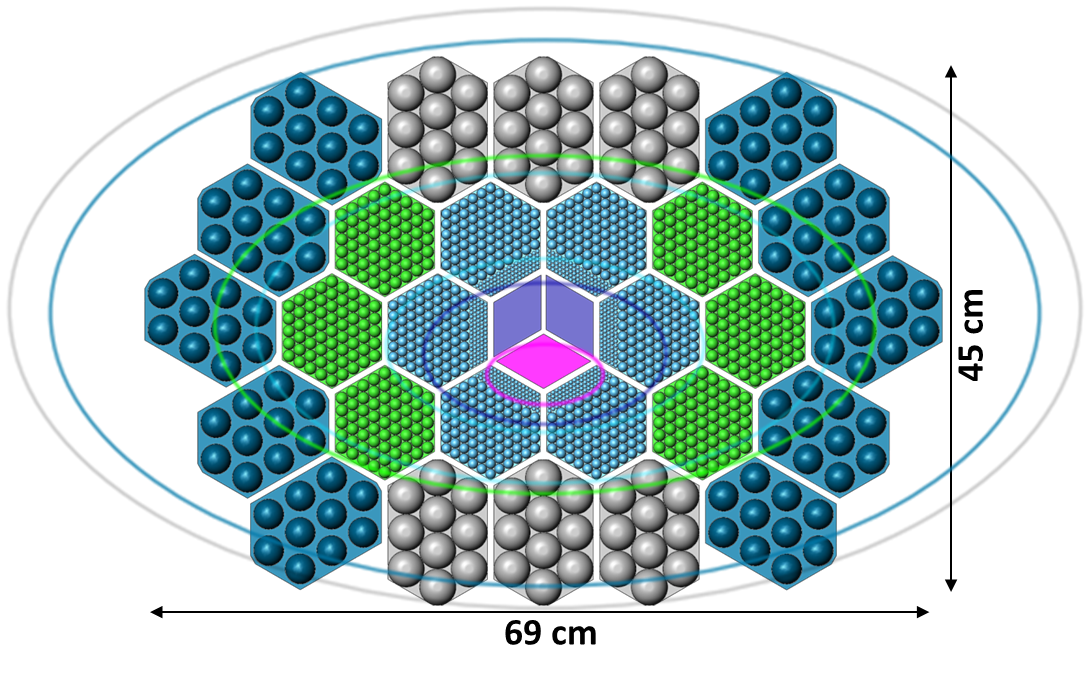
\includegraphics[height=7.5cm]{version3_focal_plane.png}
%\end{tabular}
\end{center}
\caption { \label{fig:focal_plane} 
PICO focal plane layout with Strehl~$=0.8$ contours for each pixel type. The pixel and Strehl contour colors match the band colors, A-I, 
in Figure~\ref{fig:bands} }
\end{figure} 

Differencing detectors sensitive to orthogonal polarization states will enable each pixel to make a measurement of 
a particular Stokes parameter. Pixels sensitive to the $U$ Stokes parameter were rotated by 45~deg relative to those
that were sensitive to $Q$. This Q/U measurement was in the instrument reference frame with the $x$-axis parallel to the scan 
direction; see Figure~\ref{fig:QU}.  \comr{combine Figures 6 and 7 together?}

\begin{figure} [ht]
\begin{center}
%\begin{tabular}{c} %% tabular useful for creating an array of images 
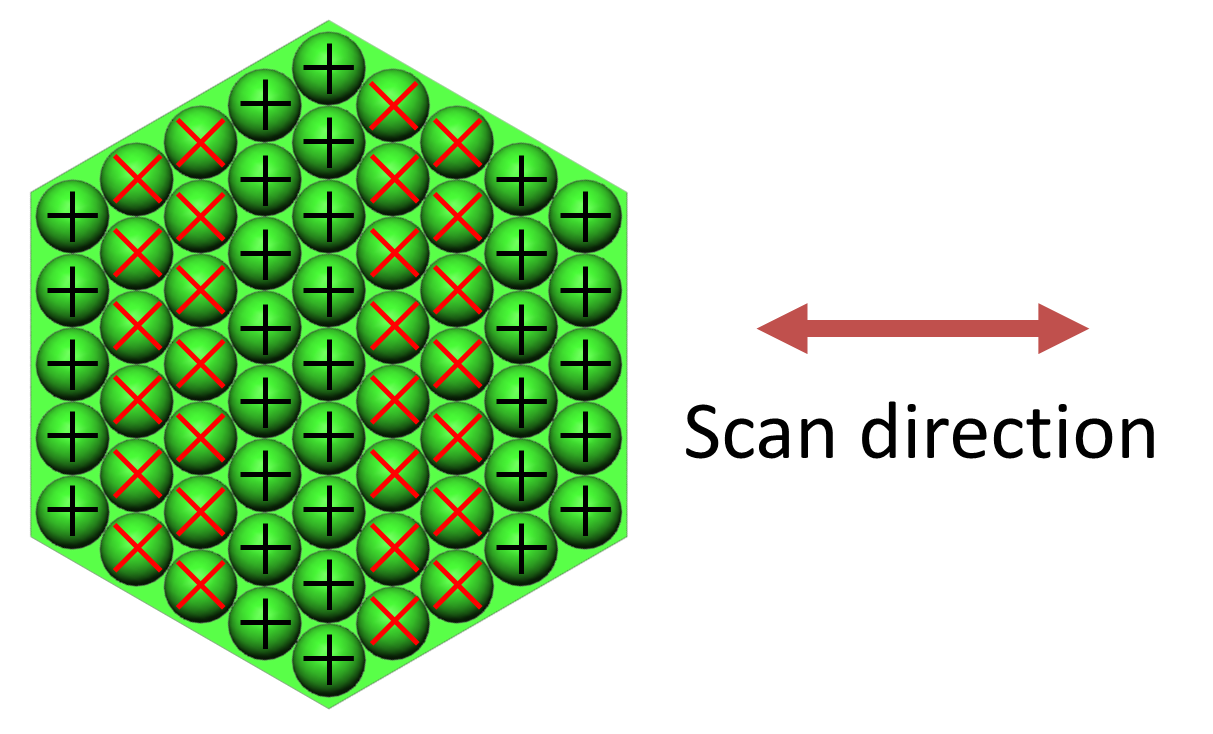
\includegraphics[height=4cm]{QU_wafer.png}
%\end{tabular}
\end{center}
\caption { \label{fig:QU} 
Layout of pixels sensitive to Stokes Q (black crosses) and Stokes U (red exes) for an example wafer.}
\end{figure}

The PICO focal plane readout was designed around $\times$128 time domain multiplexing (TDM), but this choice was not a 
significant driver for the focal plane layout or overall noise budget. 


\section{INSTRUMENT NOISE}
\label{sec:noise}

We developed an end to end noise model of the PICO instrument to predict full mission sensitivity and 
provide a metric by which to evaluate mission design trade-offs.  This model assumed white noise
at all frequencies. The overall sensitivity did not include calibration uncertainties or estimates of other possible 
systematic effects. To construct the model we estimated the 
optical load, calculated noise equivalent power (NEP) by source, 
combined all NEP terms to get detector noise, combined all detectors to get noise per frequency band, and then 
included total mission time to find overall mission sensitivity.\cite{suzuki2013_thesis,aubin2013_thesis}  
Each of these steps included various assumptions and design decisions, 
which are discussed in this section.  The assumptions are summarized in Table~\ref{tab:assume}.
The values presented in this section are current best case estimates. Instrument noise {\it requirements}, which would have larger 
noise levels, were still being determined.

To validate our model we compared two independent calculations using codes that were used for several earlier
CMB instruments.  The calculations agreed within 1\% for individual noise terms 
and for overall mission noise.  We also used our model to calculate CORE and LiteBIRD noise from their published system parameters. The 
results were consistent with published values when similar assumptions were used.  
\comr{move these to later; let's talk on the phone} 
%Additionally, we compare PICO detector noise to CORE and LiteBIRD detector noise.  The lower PICO noise is explained by the cold system and differing 
%optical efficiency.  
From these test we concluded that our model was correct and our assumptions were reasonable.

\begin{table}[ht]
\centering
\caption{Noise model parameters, see text for details. }
\label{tab:assume}
%
\begin{tabular}{|l|l|}
\hline
%                                 &                                                  \\
Throughput                       & single moded, $\lambda^2$          \\
Fractional Bandwidth             & 25\%                                             \\
Reflector emissivity             & $\epsilon = \epsilon_0\sqrt{\nu/\text{150~GHz}}, \epsilon_0 = 0.07\%$ \\
Aperture stop emissivity         & 1                                                \\
Low pass filter reflection loss  & 8\%                                                \\
Low pass filter absorption loss$^a$  & frequency dependent, 0.2\%--2.8\%             \\
Bolometer absorption efficiency  & 70\%                                             \\
T$_e$ of low, middle, and high bands (dB) & 4.8, 10.0, 20.7                                               \\
$\eta_{\rm stop}$ of low, middle, and high bands & 0.68, 0.90, 0.99   \\
Bose noise fraction, $\xi$       & 1                                                \\
Bolometer yield                 & 90\%                                             \\
Bath temperature, $T_o$ (mK)    & 100                                              \\
TES critical temperature, $T_c$ (mK)   & 187                                              \\
Safety factor, P$_{\rm sat}$/P$_{\rm abs}$      & 2                                                \\
Thermal power law index, $n$    & 2                                                \\
Intrinsic SQUID noise (aW/$\sqrt{\text{Hz}}$)   & 3                        \\
TES operating resistance, $\Omega$    &  0.03                               \\
TES transition slope, $\alpha$    & 100                                         \\
TES loop gain                    & 14                                \\
Mission length (years)           & 5                                                \\
Observing efficiency             & 95\%                                             \\
%Multiplexing factor              &
%Number of rows/columns/whichever matters . .. 
%\comr{other?}                    &                                                  \\
\hline
\multicolumn{2}{l}{\footnotesize $^a$Assumes different thickness per pixel type.}
\end{tabular}
\end{table}


\subsection{Single bolometer noise}
\label{sec:det_noise}

\subsubsection{Model}

The sources of optical load were the CMB, the primary and secondary reflectors, the aperture stop, and low pass filters.  
These elements are shown schematically in Figure~\ref{fig:load}. 
The total load absorbed at the bolometer was the sum of the power emitted by each element reduced by the transmission 
efficiency of the elements between the emitting surface and the bolometer.  
The absorbed power was
\begin{equation}
\label{eq:load}
P_{\rm abs} =  (((( P_{\rm CMB} \eta_{\rm PRI} + P_{\rm PRI} ) \eta_{\rm stop} + P_{\rm stop}(1-\eta_{\rm stop}) ) \eta_{\rm SEC} + P_{\rm SEC})\eta_{\rm filter} + P_{\rm filter}) \eta_{\rm bolo},
\end{equation} 
where $P_{\rm elem}$ is the in band power emitted by a given element for a single polarization and $\eta_{\rm elem}$ is the 
transmission efficiency 
of the element. Power emitted by the stop was a special case. We multiplied $P_{\rm stop}$ by 
$(1-\eta_{\rm stop})$ because $\eta_{\rm stop}$ is the spillover efficiency, the fraction of the throughput passing through the 
stop. Therefore $(1-\eta_{\rm stop})$ is the fraction of the throughput which views the stop. We determined 
$\eta_{\rm stop}$ in the following way. 
The MCP angular beam width depends on the wavelength and pixel diameter as\cite{suzuki2013_thesis}
\begin{equation}
\label{eq:mcp_beam}
\theta_{1/e^2} = \frac{2.95 \lambda}{\pi D_{\rm px}}. 
\end{equation} 
We fixed $D_{\rm px}$ such that 
the edge taper, T$_e$, of the middle frequency band in each pixel was 10~dB and calculated T$_e$ for the upper and lower bands 
using Equation~\ref{eq:mcp_beam}. This changing illumination of the stop is shown schematically by 
the dashed rays in Figure~\ref{fig:load}. 
For each MCP in pixels A-H, T$_e$ was 4.8, 10, and 20.7~dB for the lower, middle, and upper bands, respectively.  These 
edge tapers corresponded to $\eta_{\rm stop}$ of 0.68, 0.90, and 0.99.
The changing $\eta_{\rm stop}$ had two main effects; changing optical efficiency between bands, which affected optical load 
and the NEP to noise equivalent temperature (NET) conversion, and telescope beam size not scaling smoothly with $\lambda$.
The left panel of Figure~\ref{fig:popt} gives the optical load as a function of frequency. The jumps in load between 
neighboring bands near 70 and 200~GHz, were 
due to $\eta_{\rm stop}$ changing with frequency, which was a consequence of using MCPs. 

\begin{figure} [ht]
\begin{center}
%\begin{tabular}{c} %% tabular useful for creating an array of images 
\hspace{1cm} 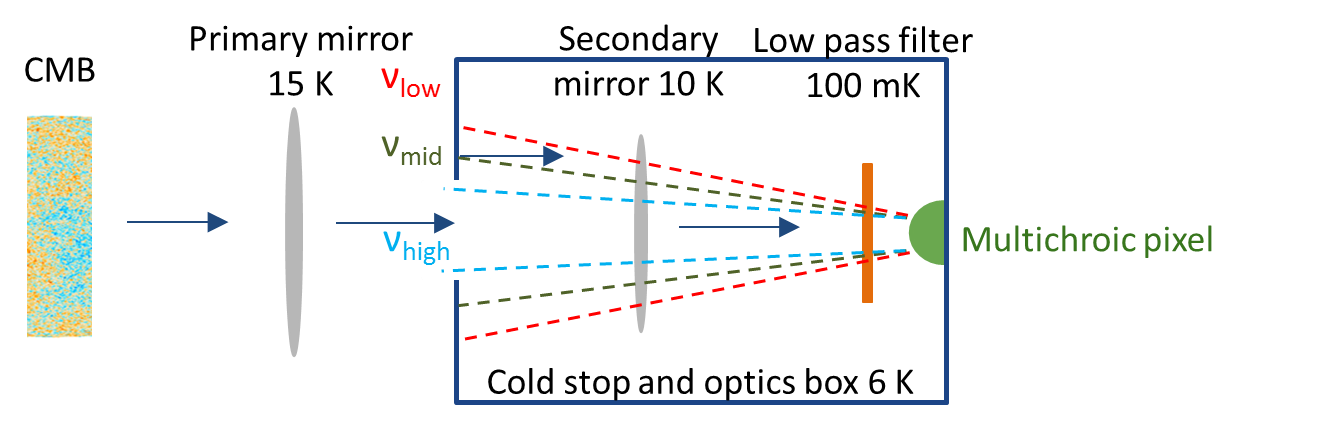
\includegraphics[height=5cm]{load_calc_MCP.png}
%\end{tabular}
\end{center}
\caption[load] { \label{fig:load} 
Schematic representation of the prediction of optical load.  Power emitted by each element was modified by the efficiency of 
the following elements and added to the total expected load.  The multichroic pixel illuminated the stop differently for 
each of the three bands. }
\end{figure} 


\begin{figure} [ht]
\begin{center}
\begin{tabular}{ccc} %% tabular useful for creating an array of images 
%\includegraphics[height=8cm]{P_optical.png}
\hspace{-1.4cm} 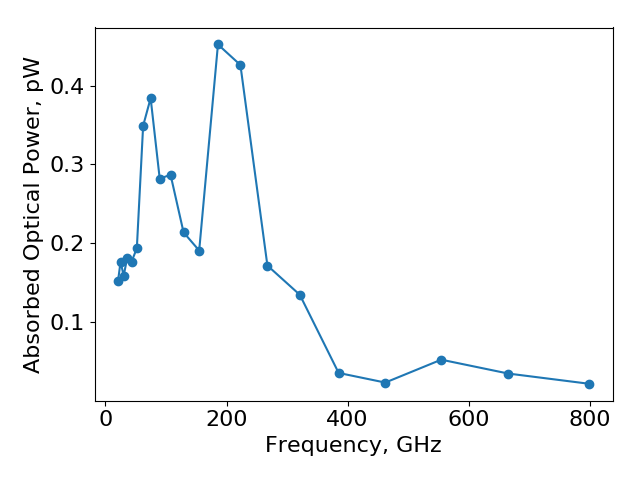
\includegraphics[height=4.9cm]{system_Popt.png} & \hspace{-0.7cm} 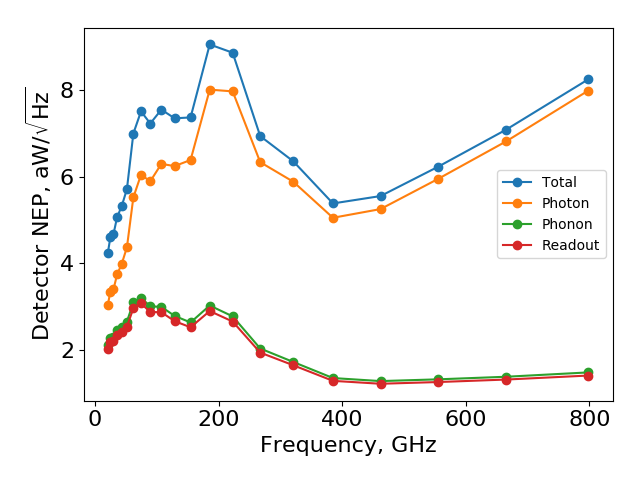
\includegraphics[height=4.9cm]{system_NEP.png} &\hspace{-0.7cm}  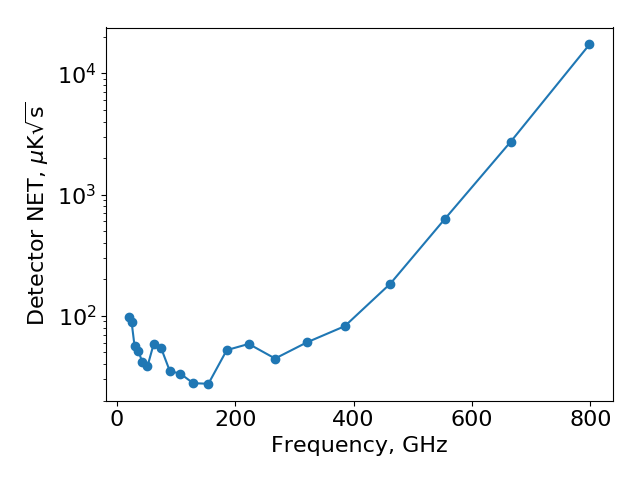
\includegraphics[height=4.9cm]{system_NET.png} 
\end{tabular}
\end{center}
\caption{ \label{fig:popt} \label{fig:noise} \label{fig:net} 
Left: Expected optical load as a function of frequency for single polarization PICO bolometers. 
Center: Breakdown of NEP sources across the PICO frequency range.  Photon noise dominates even at the lowest frequencies. 
Right: Single detector NET for the PICO bands. 
}
\end{figure} 

We considered four noise sources per bolometer; photon, phonon, TES Johnson, and readout. 
Photon noise depends on the absorbed power\cite{richards1994}, 
\begin{equation}
\label{eq:photon}
NEP_{\gamma}^2 = \int\limits_{\rm band} 2h\nu p_{\nu} \, d\nu + 2\xi \int\limits_{\rm band} p_{\nu}^2 \,  d\nu,
\end{equation} 
where $p_{\nu}$ is the power spectral density for a single polarization absorbed at the bolometer and $\xi=1$ is the fraction of correlated Bose 
photon noise. We included a factor of 2 in the Bose noise term because the bolometers received power from a single 
polarization. 
From $P_{\rm abs}$ we calculated the TES bolometer properties and phonon noise.\cite{mather1982}  
We calculated TES Johnson noise, which depended on bolometer bias parameters, for each frequency band.  
All noise sources in the cold and warm readout electronics were lumped under the readout term.  The combined NEP and the NEP per noise source are shown in 
Figure~\ref{fig:noise} as a function of frequency; the combined values are given in Table~\ref{tab:noise}.

\subsubsection{Results}  

The primary contributor to noise was the optical load. The CMB and stop accounted for the majority of the optical load 
at all frequencies. Even at 800~GHz the CMB and stop
accounted for 12\% more power than the reflectors;  \comr{show components in the Figure?} \como{This is not really feasible in the availible time. We can just quote the numbers and remove `see the left . . .'}
see the left panel of Figure~\ref{fig:popt}.
\comr{is the following consistent with the previous sentence?} \como{Yes. (fraction from CMB + stop) / (fraction from reflector) = 53/47 = 1.12} 
The load from the reflectors was greatest at 799~GHz where it was 47\% of the total 
optical load. The CMB provided more than half the load 
in the middle and upper bands of the multichroic pixels, but the stop dominated the load in the lowest band of each pixel.  
Load from the stop in the lowest band of each pixel ranged from 1.2 times the CMB load at 21~GHz to a maximum of 4.7 
times the CMB load at 223~GHz. \comr{did we consider two bands per pixel?} \como{Did we consider dual-chroic pixels in the design phase? No, or at least not in any quantitative detail.}

Bose noise was most significant 
at lower frequencies with NEP$_{\rm Bose}$/NEP$_{\rm Poisson}= 1.5 $ in the lowest band. (All NEP ratios were calculated using 
units of W/$\sqrt{\rm Hz}$ for the dividend and divisor.)  However, Poisson noise increased as 
$\sqrt{P_{\rm abs}\nu}$ while Bose was proportional to $P_{\rm abs}$. Poisson noise equaled Bose noise at 30~GHz and dominated at higher bands; 
NEP$_{\rm Bose}$/NEP$_{\rm Poisson} <10\%$ at 321~GHz. 
Phonon noise was the second most significant source, NEP$_{\rm phonon}$/NEP$_{\rm photon}$ ranged from 65\% at 21~GHz 
to 19\% at 799~GHz. 
% this is NEP/NEP NOT squared.  Squared is 2.2 at 21 GHz and 0.01 at 321. < 10 at 129 GHz.  in NEP to NEP bose = poisson at 30 GHz

For TDM readout, phonon and readout noise were approximately equal with TES Johnson noise being insignificant.  We also modeled 
noise for frequency domain multiplexing readout (FDM).  For FDM the TES Johnson noise was higher, 2/3 of the readout NEP, but the readout 
noise was lower.  Comparing the combined TES Johnson and readout NEPs for TDM and FDM we founnd essentially identical performance 
with total noise differing by less than 3\% across all bands.  For both systems we required a focal plane temperature, $T_o$, of 
100~mK and a bolometer safety factor of 2 to remain photon noise dominated at the lowest bands. \comr{what does this mean? that 
if the safety factor is higher we are not photon noise dominated?} \como{Yes. At safety factor 2.5 phonon noise is larger than photon at 21 GHz.} 
%\comr{should we have Dobbs review this?} \como{I don't think it is necessary. But you're more familiar with the politics of this one. Dobbs isn't a co-author, if that matters.}

\subsection{Combined  array noise}

Using single detector NEPs from Section~\ref{sec:det_noise} and the detector counts from Section~\ref{sec:focalplane} we 
calculated the combined NEP of the detector array for each band.  Combining detectors simply reduced noise by $\sqrt{N}$ 
except for Bose photon noise. 
For the lowest band of each MCP the pixel spacing was $0.4$F$\lambda$ and thus the pixels oversampled the point spread function leading 
to correlated photon noise between pixels.
Accounting for this effect gave a 26\% increase in the combined array NEP for the 21~GHz band 
and a 0.003\% increase at 799~GHz.  

From the array NEP we converted to noise equivalent temperature (NET) per band using
\begin{equation}
\label{eq:NET}
\frac{NEP}{NET} = \sqrt{2} \, \eta_{\rm opt} \int\limits_{\rm band}\frac{dp_{\nu}}{dT}\Bigr|_{T_{\rm CMB}} d\nu.
\end{equation} 
The $\eta_{\rm opt}$ term contributed to the `jumps' in $NET$ seen in Figure~\ref{fig:net}, because $\eta_{\rm opt}$ varied band to band.  
Numerical values for the NET are given in the second to last column in Table~\ref{tab:noise}.

Assuming evenly weighted observations 
of the full sky, 5 years of mission duration, and 95\% efficiency, we calculated full mission map sensitivities in polarization; see the 
final column in Table~\ref{tab:noise}. 
Combining all bands gave a total CMB map depth for the entire PICO mission of 0.62~$\mu$K$_{\rm CMB}$-arcmin.

\begin{table}[ht]
\centering
\caption{PICO frequency channels and noise. }
\label{tab:noise}
\begin{tabular}{|c|c|c|c|c|c|c|cc|}
\hline
Pixel  & Band  & FWHM   & Bolometer NEP & Bolometer NET        & N$_{\rm bolo}$ & Array NET            & \multicolumn{2}{|c|}{Polarization map depth}  \\
Type   & GHz   & arcmin & aW/$\sqrt{Hz}$ & $\mu$K$_{\rm CMB}\sqrt{s}$ &           & $\mu$K$_{\rm CMB}\sqrt{s}$ & $\mu$K$_{\rm CMB}$-arcmin & Jy/sr     \\ \hline
A     & 21  & 38.4 & 4.89  & 112.2   & 120   & 13.6  & 19.2  & 6.69 \\
B     & 25  & 32.0 & 5.33  & 103.0   & 200   & 9.56   & 13.5 & 7.98  \\
A     & 30  & 28.3 & 4.92  & 59.4    & 120   & 5.90   & 8.31 & 7.93   \\
B     & 36  & 23.6 & 5.36  & 54.4    & 200   & 4.17   & 5.88 & 9.59   \\
A     & 43  & 22.2 & 5.33  & 41.7    & 120   & 4.01   & 5.65 & 13.9   \\
B     & 52  & 18.4 & 5.73  & 38.4    & 200   & 2.86   & 4.03 & 16.8   \\
C     & 62  & 12.8 & 8.29  & 69.2    & 732   & 3.13   & 4.42 & 37.0   \\
D     & 75  & 10.7 & 8.98  & 65.4    & 1020  & 2.47   & 3.47 & 48.1   \\
C     & 90  & 9.5  & 7.76  & 37.7    & 732   & 1.49   & 2.10 & 44.5   \\
D     & 108 & 7.9  & 8.18  & 36.2    & 1020  & 1.21   & 1.70 & 57.0   \\
C     & 129 & 7.4  & 7.35  & 27.8    & 732   & 1.09   & 1.53 & 69.7   \\
D     & 155 & 6.2  & 7.36  & 27.5    & 1020  & 0.91   & 1.28 & 84.6   \\
E     & 186 & 4.3  & 12.30 & 70.8    & 960   & 2.52   & 3.54 & 383    \\
F     & 223 & 3.6  & 12.70 & 84.2    & 900   & 3.05   & 4.29 & 579    \\
E     & 268 & 3.2  & 8.55  & 54.8    & 960   & 1.87   & 2.62 & 369    \\
F     & 321 & 2.6  & 8.16  & 77.6    & 900   & 2.73   & 3.84 & 518    \\
E     & 385 & 2.5  & 4.54  & 69.1    & 960   & 2.35   & 3.31 & 318    \\
F     & 462 & 2.1  & 4.00  & 132.6   & 900   & 4.66   & 6.56 & 403    \\
G     & 555 & 1.5  & 6.47  & 657.8   & 440   & 33.1   & 46.5 & 1569  \\
H     & 666 & 1.3  & 5.74  & 2212    & 400   & 117    & 164  & 1960 \\
I     & 799 & 1.1  & 4.97  & 10430   & 360   & 560    & 816  & 2321 \\ 
\hline
Total &     &      &       &         & 12996 & 0.46   & 0.65 &   \\
\hline
\end{tabular}
\end{table}
%https://www.tablesgenerator.com/

\comr{SH Here} 
\section{CONCLUSIONS/SUMMARY}

The PICO optical system was a simple two reflector open-Dragone which we numerically optimized to maximize the DLFOV.  The addition of a 
cold aperture stop and cold reflectors minimized optical load and reduced noise.  The focal plane took advantage of the large DLFOV and MCP 
technology to implement 12996 polarization sensitive detectors in 21 bands from 21-799~GHz.  When combining all bands our instrument 
noise model predicted a full mission polarization map depth of 0.62~$\mu$K$_{\rm CMB}$-arcmin.


% \begin{itemize}
% \item Total full sky map sensitivity, compare to Planck, LB, and S4? or do so in intro?
% \end{itemize}
% simple telescope. low noise? low systematics? - systematics not discussed elsewhere (yet)


% some of this phrasing here.
% From this analysis we see that all noise sources depend on $P_{abs}$, either directly or through how load drives bolometer properties.  
% Therefore the 
% most straightforward way to reduce noise is to limit all optical loads other than the CMB.  This motivates the simple, few element telescope we 
% have designed with the aperture stop and secondary mirror actively cooled to reduce excess load and photon noise. 


\section{ACKNOWLEDGMENTS}

This Probe mission concept study is funded by NASA grant \#NNX17AK52G.  Gianfranco de Zotti acknowledges financial support from the ASI/University of
Roma--Tor Vergata agreement n.\; 2016-24-H.0 for study activities of the Italian cosmology community. Jacques
Delabrouille acknowledges financial support from PNCG for participating to the PICO study.


\bibliographystyle{spiebib} % makes bibtex use spiebib.bst
\bibliography{refs} % bibliography data in refs.bib


\end{document} 


% LocalWords:  PICO
